% GitHub cvitanov/reducesymm/tingnan/dailyBlog.tex

% Predrag                                       2014-04-18
	
\chapter{Research blog on matters diffusive}
\label{c-DailyBlog}




\begin{description}

\item[2014-05-20 Predrag]
We can write up the narrative starting with this file,
in this folder, \texttt{reducesymm/tingnan/},
with all stuff that does not belong to the public version
bracketed by \texttt{ifboyscout}...\texttt{fi} .
You can clip \& paste anything from here or from
ChaosBook.org, if that saves you LaTeXing time.

\item[2013-02-03 Roberto]
incorporate kneading determinants from
G.~Cristadoro\rf{Cristad06}
{\em Fractal diffusion coefficient from {\dzeta}s}.

\item[2009-02-27 Predrag]
Read  Gilbert  and Lefevere\rf{GilbLef08},
    ``Heat conductivity from molecular chaos hypothesis
             in locally confined billiard systems,''

``From Deterministic Chaos to Deterministic Diffusion''
by R. Klages, \arXiv{0804.3068}: ``
A set of easy-to-read lecture notes for a short first-year Ph.D.
student course. The notes cover five hours of lectures and
do not require any prior knowledge on dynamical systems. The first part introduces
to deterministic chaos in one-dimensional maps in form of Lyapunov exponents
and the metric entropy. The second part first outlines the concept of
deterministic diffusion. Then the escape rate formalism for deterministic
diffusion, which expresses the diffusion coefficient in terms of the above two
chaos quantities, is worked out for a simple map. The notes conclude with a
very brief sketch of anomalous diffusion.

For `fundamental domain' in hyperbolic geometry, see for example
\HREF{http://www.math.ou.edu/~kmartin/mfs/ch3.pdf}{these notes}
by \HREF{http://www.math.ou.edu/~kmartin}{Kimball Martin}.

\item[2014-02-27 Predrag] Must read:
Dettmann\rf{Dettm14}, {\em Diffusion in the {Lorentz} gas}.
Georgie Samuel Knight {\em Fractal Diffusion Coefficients in Simple
Dynamical Systems}
\HREF{http://www.maths.qmul.ac.uk/~klages/people/knight_phd_final.pdf}
{PhDthesis} (2012) might also be helpful.

generate \texttt{f\_diff\_MarkPart.pdf}
from \texttt{.../xfig/f\_diff\_MarkPart.fig}

\item[2013-02-28 Predrag] to Tingnan Zhang:
Dettmann's review, \arXiv{1402.7010} is something that you want to read -
looks very complete. {\bf Goldman:} Sects. 7.4 and 7.5 and refs within
are tantalizing.

\item[2013-03-25 Predrag] to Tingnan Zhang:
{\em Superdiffusion in the periodic Lorentz gas} by
Jens Marklof and Balint Toth,  	\arXiv{1403.6024} is too mathematical and
general for our purposes (hopefully we will have no super-diffusivity, noise
should wipe that out), but
Sect.~2~{\em The scattering map} might be useful for your exposition
(or its prequel  \arXiv{0801.0612}).

\item[2014-04-18 Predrag]
Sinai\rf{Sinai04} might be a quick read.
Recent references of possible interest:
Zhang\rf{HKZhang11}
{\em Current in periodic {Lorentz} gases with twists}.

\item[2014-04-18 Predrag]
I have saved the Lorentz\rf{Lorentz1905} 1905
{\em The motion of electrons in metallic bodies}
(\HREF{http://chaosbook.org/library/Lorentz1905.pdf}{click here}).

\item[2014-04-18 Predrag]
For great wallpapers, see overheads in
\HREF{http://www-personal.umich.edu/~engelmm/lectures/ShortCourseSymmetry.html}
{Engel's} course.

\item[2014-04-18 Predrag]
Dresselhaus \etal\ textbook\rf{Dresselhaus07}
(\HREF{http://chaosbook.org/library/Dresselhaus07.pdf}{click here})
is good on discrete
and space (but not continuous) groups.
The MIT~course~6.734
\HREF{http://stuff.mit.edu/afs/athena/course/6/6.734j/www/group-full02.pdf}
{online version} contains much of the same material.

Chapter {\em 9. Space Groups in Real Space} is quite clear on matrix
representation of space groups. The translation group $T$ is a normal
subgroup of \Group\ and defines the Bravais lattice. The cosets by
translation $T$ (set all all group elements obtained by all translations)
form a factor group $\Group/T$, isomorphic to the point group $g$
(rotations). All irreducible representations of \Group\ can be compounded
from irreducible representations of $g$ and $T$.

Section {\em 9.3 Two-Dimensional Space Groups}: In the international
crystallographic notation, our hexagonal lattice \#17 is called $p6mm$,
with point group $6mm$.
\[
g = \{
E, C_6^+, C_6^-, C_3^+, C_3^-, C_2,
\sigma_{d1}, \sigma_{d2}, \sigma_{d3},
\sigma_{v1},\sigma_{v2}, \sigma_{v3}
\}
\]
Prefix $p$ indicates that the unit cell is primitive (not centered). This
is a simple or {\em symmorphic} group, which makes calculations easier.
The Bravais lattice is two equilateral triangles, not sure how to relate
it to our hexagonal `elementary cell'? A Brilloun zone? Bravais `unit cell'
is illustrated in Fig.~E.2. ChaosBook `Fundamental
domain' makes an appearance in Fig.~10.2.

The main trick in quantum-mechanical calculations is to go to the
\emph{reciprocal} space (see Fig.~E.2), in our case with the full
$\Gamma$ point, $k=0$, wave vector symmetry (see Table~10.1), and `Large
Representations'. This is something we have not tried in deriving the
trace formula for deterministic diffusion.

Sect. {\em 10.5 Characters for the Equivalence Representation} look
like those for the point group, sort of. We should probably work
out problems 10.1 and 10.2.

\item[2014-04-24 Tingnan]
Remember that some orbits that lie on the boundary of fundamental domain
have only 6 copies.

\item[2014-04-26 Predrag]
All divisors of 12 are possible multiplicites. The fully symmetric state
of multiplicity 1 would be an \eqv\ point at the origin: possible for
soft potentials but not for this billiard. Rest you can easily doodle if
you draw the hexagonal lattice (disks replaced by point): there is \po\
of length 6 (edges of the hexagon) of multiplicity 2 (the two
orientations of the orbit), and there should be orbits of multiplicity 3,
4, 6 and the generic asymmetric orbits of multiplicity 12.

\item[2014-04-24 Pavel]
Tingan and I have realized that in a
pseudo-cycle it is possible to have two or more prime cycles that differ
by a group action. In some sense, cross-terms still disappear, but it is
impossible to assign unique weights to each fundamental domain cycle.

\item[2014-04-26 Predrag to Tingan]
After the project is delivered,
have a look at
Knauf\rf{Knauf87,AschKnauf97},
{\em Ergodic and topological properties of {Coulombic} periodic potentials},
{\em Motion in periodic potentials},
Baldwin\rf{Baldwin88} {\em Soft billiard systems},
Kimball\rf{Kimball01}
{\em Chaotic properties of the soft-disk {Lorentz} gas},
B\'alint and T\'oth\rf{BaTo03,BaTo04}
{\em Correlation decay in certain soft billiards},
{\em Mixing and its rate in `soft' and `hard' billiards
         motivated by the {Lorentz} process},
and
Elyutin\rf{Elyutin04}
{\em Lyapunov exponent for a gas of soft scatterers}.
Blog about relevant parts here, if there is something of interest
to us.

\item[2014-04-26 Predrag] We should read Chapter 7 of Gaspard\rf{PG97}.
Kimberly and I both have a hard copy. Gaspard discusses irreps of
the translation group in some detail.

\item[2014-04-26 Predrag]
I'm quite convinced that this problem is a solved problem, we just have
to understand how characters are used to project irreps of space groups.
One has to go to the reciprocal lattice, and utilize utilize the concept
of the `star'. All physical chemists and crystallographers know how to do
this - we just need to be good students and read the stuff. Our case is
the most symmetric, $p6mm$ lattice - it is surely worked out in some
paper in a way that we can understand. They call our `fundamental domain'
the `motif' or the `asymmetric unit'.

I found projects in \HREF{http://www-f1.ijs.si/~ziherl/SF.html} {this
course} easy to read, especially Toma\v{z} \v{C}endak, who reviews the
space groups theory in a pretty simple way, and Zavadlav has very pretty
wallpaper groups illustrations. Ziherl recommends Elliott and  Dawber,
{\em Symmetry in Physics}\rf{ELLIOTT}.

Joseph Sidighi likes Cotton\rf{Cotton08} {\em Chemical applications of
group theory}, which has no characters for space groups, but a very
pretty discussion of their geometry in Chapt.~11. Cotton was ``the most
influential inorganic chemist to ever have lived.''

If we succeed in factorization, this would merit a publication.
It is OK if you do not succeed in factorization - I have failed myself, so
who am I to cast the first stone:)

\item[2014-05-02 Predrag]
Pavel again has an idea. Forget the translation group; tile every Lorentz
gas orbit by the little triangles (copies of the fundamental domain,
1/12th of the elementary cell). Then the group orbit is generated by 3
elements (ignoring going through the corners): go to the domain to the
left/right (generators of \Dn{12}) and flip the domain so it leaves the
elementary cell. To Predrag this is reminiscent of Penrose tailings,
where the space is tiled without the translations over square or cubic
lattice. For that, Mermin's article\rf{Mermin92} on space groups of
quasicrystals might be of interest.

I think the idea should be worked out in one dimension first, but Pavel
thinks that would be too simple. Predrag believes that you always work
out the simplest model first. $\ExpaEig =2$ vanishes by eq.~(25.20)
(\HREF{http://www.streamsound.dk/book1/chaos/chaos.html\#535/z} {click
here}), so the simplest diffusion models are for $\ExpaEig =3$ or $4$.
Reduce the map to the fundamental domain (positive 1/2 line) as in
ChaosBook fig.~9.8: The bimodal Ulam sawtooth map
(\HREF{http://www.streamsound.dk/book1/chaos/chaos.html\#186/z} {click
here}). That should give the symmetry-reduced symbolic dynamics, but the
group is larger than \Dn{1}, which works `within the elementary cell', by
generating the negative axis copy of the fundamental domain: one adds a
reflection that flips the flips the fundamental domain (the half-unit
interval) outside of the elementary cell, to the adjoining tile (the
second one to the left or the right. This operation generates the
translations, and together the two group operations assign a symbolic
itinerary to any orbit. Then one should find the rule that reads of the
global translation from the symbolic itinerary, insert this into the
cycle expansions for the deterministic diffusion formula.

For $\ExpaEig =2$ I get that the fundamental domain dynamics is given by
the full tent map
(\HREF{http://www.streamsound.dk/book1/chaos/chaos.html\#244/z} {click
here}), so it cannot be simpler. Too bad that $D=0$ identically :)

\item[2014-05-03 Predrag] I drew by hand the $\Dn{1}$ reduction of the
dynamics to the fundamental domain for $\ExpaEig =3$ case - it is really
simple and it works. Guys, try it, then try it for the Lorenz gas. I'm
optimistic.

\item[2014-05-03 Predrag] Pavel is right - 1D case is probably
misleading, I used only translations to find the global displacement.
With reflections, the distances on the 2D lattice corresponding to
relative prime cycles will not be integer vectors - their construction
will resemble what we do when we bounce a straight trajectory off a
sequence of 3-disks, it will be a computation, and go to the new
`comoving' coordinate frame. But a doable one. Maybe one should play with
the least symmetric triangular $p3$ ($\Zn{3}$ point group) tiling first,
rather than with the most symmetric hexagonal $p6mm$ lattice ($\Dn{6}$
point group).

\item[2014-05-05 Tingnan] My numbers of elementary cell prime cycles,
Lyapunov exponents and diffusion coefficients are listed and compared
to the Schreiber calculation in \reftab{TCELL1}. I still have the problem
for the convergence of diffusion coefficients. Did we miss a factor of 2
somewhere?

\begin{table}
\begin{center}
\begin{tabular}{|r|r|l|l|l|}
\hline
length & \# cycles & $\zeta$(0,0) & $\lambda$ & D \\ \hline\hline
1      & 0      &   -    &   -  &   - \\
2      & 24     & -0.31697 & 1.330 & 0.750\\
3      & 64     & -0.54152 & 1.435 & 0.677\\
4      & 156    & -0.09718 & 1.902 & 0.565\\
5      & 492    &  0.02383 & 2.324 & 0.425\\
6      & 1484   &  0.02812 & 1.931 & 0.259\\
7      & 5244   &  0.02044 & 1.836 & 0.371\\
8      & 19008  & -0.00036 & 1.754 & 0.513\\ \hline\hline
\multicolumn{3}{|l|}{\refRef{MacZwa83}, estimate}
                           &   -   & 0.175 \\
\multicolumn{3}{|l|}{numerical experiment}
                           & 1.760 & 0.25
\\ \hline
\end{tabular}
\hfill
\begin{tabular}{|r|r|l|l|l|}
\hline
length & \# cycles & $\zeta$(0,0) & $\lambda$ & D \\ \hline\hline
1      & 0      &   -    &   -  &   - \\
2      & 24     & -0.34807 & 1.312 & 0.759\\
3      & 64     & -0.57736 & 1.418 & 0.686\\
4      & 168    & -0.11233 & 1.908 & 0.571\\
5      & 517    &  0.01373 & 2.406 & 0.407\\
6      & 1582   & -0.01062 & 1.998 & 0.227\\
7      & 5387   & -0.01084 & 1.900 & 0.333\\
8      &        &          &       &       \\
\hline\hline
\multicolumn{3}{|l|}{     }& ?.??? & ?.??? \\
\multicolumn{4}{|l|}{numerical experiment} & 0.25 \\ \hline
\end{tabular}
\caption{\label{TCELL1}
Elementary cell, $w$=0.3.
(left) Schreiber 1992 calculation\rf{CGS92}.
Gaspard 1992 note:: ``My numerical estimate for the Lyapunov exponent
when $w=0.3$ is $\lambda = 1.760 \pm 0.002$, which supports the result of
this table.''
(right) Zhang 2014-05-05 calculation.
}
\end{center}
\end{table}

\item[2014-05-07 Predrag]
Note that while Tingnan more prime periodic orbits than Thomas Schreiber,
convergence is not improved. To the contrary: the diffusion constant and
the Lyapunov exponent of \reftab{TCELL1} do not agree for even $\cl{}=2$,
so something is seriously amiss. It is unlikely that Thomas and
I would have gotten that wrong. Have to
\begin{enumerate}
  \item  Please create
  \reftab{tabListLength2} for the 24 cycles of length $\cl{}=2$ with
  (a) symbolic dynamics (see \refTab{TSYM}),
  (b) $\ExpaEig_p$,
  (c) $\period{p}$, and
  (d) $\hn_t(x)$, the discrete lattice translation \refeq{hatn}.
  \item
  Check the $\ExpaEig$'s, $\period{}$'s of the shortest ones, the ones
  that are the same as for the 3-disk billiard, against the analytical
  expressions given as exercises in ChaosBook,
(\HREF{http://www.streamsound.dk/book1/chaos/chaos.html\#300/z}
{click here}).
  \item
Verify that Tingnan's implementations of \refeq{TS:formula} and
\refeq{TS:eqliap} have been correctly coded.
  \item \reftab{TCELL}
\end{enumerate}


\begin{table}
\begin{center}
\begin{tabular}{|c||r|r||c|c|}
\hline
symbol & \multicolumn{2}{|c||}{amount of change} &
 \multicolumn{2}{|c|}{direction of change} \\
       & last long & last short & next the same & next other way \\ \hline
a      &    1      &     2      &     x      &       \\
b      &    3      &     4      &     x      &       \\
c      &    5      &     6      &     x      &       \\
d      &    5      &     4      &            &   x    \\
e      &    3      &     2      &            &    x   \\
f      &    1      &     -      &            &    x   \\ \hline
A      &    2      &     1      &     x      &       \\
B      &    4      &     3      &     x      &       \\
C      &    6      &     5      &     x      &       \\
D      &    4      &     5      &            &    x   \\
E      &    2      &     3      &            &    x   \\
F      &    -      &     1      &            &    x   \\ \hline
\end{tabular}
\caption{\label{TSYM}
Symbols in the fundamental domain.}
\end{center}
\end{table}

\input tabListLength2

\item[2014-05-05 Tingnan]
\refFig{KimFig2} is taken from the Kimball article\rf{Kimball01} on soft
    billiards. Let $\b_i$ and $\phi_i$ be the impact parameter and
    propagation angle(in the global frame) before i-th collision. We
    can then compute the monodromy matrix. Suppose the scattering
    funtion is provided by $\theta(b)$, we have:
    \PC{2014-05-05 promising start. Go on :)}
\[
\phi_{j+1} = \phi_j + \theta_j(b_j);
\]


\begin{figure}
\begin{center}
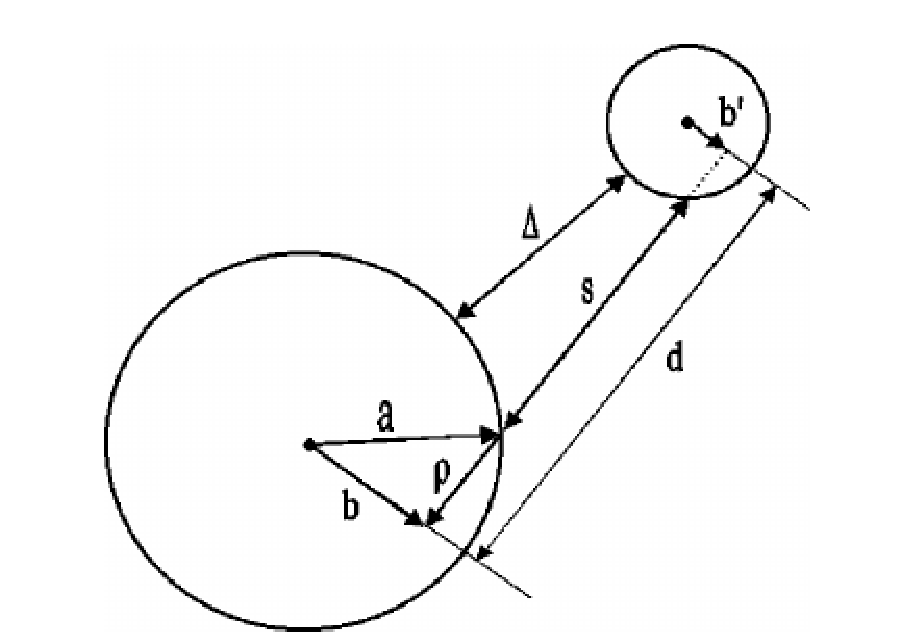
\includegraphics[width=0.45\textwidth]{Kim01_Fig2}
\end{center}
\caption{
	A portion of a path;
}
\label{KimFig2}
\end{figure}

\item[2014-05-12 Predrag to Tingnan]
We need to create our own version of Fig.~4 of \refref{CGS92}.


\item[2014-05-16 Tingnan] I listed my cycles of topological
    length 2 in \reftab{tab:ListLength2}. In \reftab{tab:comparison0}
    and \reftab{tab:comparison1} the results from numerical program are
    compared with exact formula. I will create the new figure.

\item[2014-05-18 Predrag to Tingnan] Thanks for checking - your
    numerics is 100\% good, great. I reformatted
    \reftab{tab:ListLength2} - nothing important. For some reason the
    Floquet multipliers for the \cycle{59} set are accurate only to
    $10^{-8}$, even though your check of analytic formulas are good to
    $10^{-15}$. Not a pressing problem at the moment...

%%%%%%%%%%%%%%\item[Figure ?]%%%%%%%%%%%%%%%%%%%%%%%%%%%%%%%%%%%%%%%%%%
\begin{figure}
\begin{center}
(a)\includegraphics[width=0.29\textwidth]{diskDirectionsElCell}
(b)\includegraphics[width=0.29\textwidth]{diskDirecsElCell05}
(c)\includegraphics[width=0.29\textwidth]{diskDirecsElCell05red}
\end{center}
\caption{
Elementary cell symbolic dynamics is obtained by labeling the translation
vectors connecting the center of the current disk to the center of the
next disk.
(a) The finite horizon is here imposed by limiting jumps from the
center cell to only the short jumps (six even labels $0, 2,\cdots,10$)
and the `long jumps' (six odd labels $1, 3,\cdots,11$).
(b) Running mode \cycle{05} advances by $\hn_4$ per period.
(c) In the elementary cell this is a \po\ \cycle{05}
    of topological length 2.
    }
\label{diskDirectionsElCell}
\end{figure}
%%%%%%%%%%%%%%\item[Figure 4]%%%%%%%%%%%%%%%%%%%%%%%%%%%%%%%%%%%%%%%%%%

\item[2014-05-20 Predrag]
Elementary cell symbolic dynamics labels are not disk labels, but rather
the labels of transitions between disks along the 12 translational
vectors. In \reffig{diskDirectionsElCell} I label the
translation vectors connecting the center of the current disk to the
center of the next disk.

\item[2014-05-21 Tingnan]
I migrated my code base to cpp for
faster computing speed (in order to find periodic orbits of topological
length 8). I will try both derivative-free (Nelder-Mead) routine as well
as those methods based on derivatives. The multi-dimensional flight time
function (to be minimized) seems to have a quite complex landscape which
creates a lot of numerical difficulties. Do you know which references
have figures/tables showing the diffusion coefficient/flight time/etc as
a function of some parameters? Insofar I can only find estimations on
hard disks as a function of disk separation $w$. I am looking at this
because Dan would like to see the parameter variations and their effects,
from an experimental aspect.

\item[2014-05-20 Predrag]
All illustrations seem to be worked out for 1-dimensional maps (see
references toward the beginning of this blog). We would be the first to
compute something for Lorentz billiard, I believe.

\item[2014-05-20 Predrag]
Regarding spherical billiards for Feifei Qian: there is lots of
literature on the web, Google it (though I have not found much). Random
reference: Donnay\rf{Donnay88}
(\HREF{http://chaosbook.org/library/Donnay88.pdf}{click here}).
Programming should be easy; each orbit is a great circle. If the billiard
is a sphere with a reflecting circle drawn on, find the intersection of a
great circle with it, the specularly reflect it around the intersection
point. That seems to say that all orbits (with the exception of the
equator parallel to the billiard wall circle) are marginally stable
period 2. So we need to think of something more interesting, like 2
circular billiard walls, not symmetrically placed...

Totally unrelated:
\HREF{http://www.domerama.com/software/sketchup-3d-models/} {Sketchup}
might be fun to use.


\begin{table}
{\small
%\begin{center}
\begin{tabular}{|r|r|l|l|l|}
\hline
$\period{p}$ & \# cycles & $\zeta$(0,0) & $\lambda$ & D \\ \hline\hline
1      & 0      &   -    &   -  &   - \\
2      & 24     & -0.31697 & 1.330 & 0.750\\
3      & 64     & -0.54152 & 1.435 & 0.677\\
4      & 156    & -0.09718 & 1.902 & 0.565\\
5      & 492    &  0.02383 & 2.324 & 0.425\\
6      & 1484   &  0.02812 & 1.931 & 0.259\\
7      & 5244   &  0.02044 & 1.836 & 0.371\\
8      & 19008  & -0.00036 & 1.754 & 0.513\\ \hline\hline
\multicolumn{3}{|l|}{\refRef{MacZwa83}, estimate}
                           &   -   & 0.175 \\
\multicolumn{3}{|l|}{numerical experiment}
                           & 1.760 & 0.25
\\ \hline
\end{tabular}
\hfill
\begin{tabular}{|r|r|l|l|l|}
\hline
$\period{p}$ & \# cycles & $\zeta$(0,0) & $\lambda$ & D \\ \hline\hline
1      & 0      &   -    &   -  &   - \\
2      & 24     & -0.34807 & 1.312 & 0.379\\
3      & 64     & -0.57736 & 1.418 & 0.343\\
4      & 168    & -0.11233 & 1.909 & 0.285\\
5      & 516    &  0.01399 & 2.408 & 0.202\\
6      & 1589   & -0.01291 & 2.004 & 0.110\\
7      & 5700   & -0.02034 & 1.903 & 0.170\\
8      & 20729  & -0.00109 & 1.785 & 0.240\\
\hline\hline
\multicolumn{3}{|l|}{\HREF{arixv.org/pdf/1202.2904.pdf}{click here}}& - & 0.25 \\
\multicolumn{4}{|l|}{numerical experiment} & 0.25 \\ \hline
\end{tabular}
} %end {\small
\caption{\label{TCELL}
Elementary cell, $w$=0.3.
(left) Schreiber 1992 calculation\rf{CGS92}.
Gaspard 1992 note: ``My numerical estimate for the Lyapunov exponent
when $w=0.3$ is $\lambda = 1.760 \pm 0.002$, which supports the result of
this table.''
(right) Zhang 2014-05-23 calculation.
}
%\end{center}
\end{table}

\item[05-23-2014 Tingnan]
I think I in my and Schreiber's numerical calculation for the diffusion
coefficients we have missed the spatial dimension $\nu=2$ at the
denominator \refeq{TS:formula}. Now results are updated in
\reftab{TCELL}. Should we say that now both Lyapunov and diffusion
coefficient are converged?

\item[05-23-2014 Predrag]
Impressive calculation for $\period{}=8$!
You are right about Schreiber missing $\nu=2$; I have it in my overheads.
The number of cycles seems to be creeping
up (from initial Tingnan's \reftab{TCELL1} to the current \reftab{TCELL}.
I doubt I'll ever find the Schreiber's data, it is so long ago...

My worry is still that the diffusion constant and
the Lyapunov exponent of \reftab{TCELL1} do not agree for even $\cl{}=2$, so maybe
I'll have to recompute \refeq{TS:formula} in this case, using your
\reftab{tab:ListLength2} data.
The convergence for both the Lyapunov and the diffusion
coefficient seem not very good, but let's see well the Lyapunov works out
once you compute it in the fundamental domain.

\item[05-26-2014 Tingnan]
If I am not wrong the zeta function for $n=2$ and $n=3$ cases are just the summation over the weights (using the truncation formula)
\[
\zeta(0,0)=1-\sum_{\cl{p}\leq2,3}t_{p}=1-\sum_{\cl{p}\leq2,3} \frac{1}{\ExpaEig_{p}}
\]
I am starting to compute the cycles in the fundamental domain.
Not sure how to convert the fundamental domain symbols (a-f, A-F) into my program. Are we still trying to use the least action method in the fundamental domain? If so, for each of the symbol, which disks should be included for the computation? In Fig.~5 of Schreiber paper we can see that the number of the disks visited for each symbol
is different. And I am not sure about this sentence in Schreiber's paper:

``The right and left turns are not distinguished - instead,  one reads
off a symbol whether the next turn has to be taken in the same or in the
opposite sense."

\item[2014-05-28 Predrag] Notions `right' and `left' are well defined in
the elementary cell. In the fundamental domain on indicates only the
successive relative orientations: either one turns in the same sense as
in the preceding turn, or one turns in the sense opposite of the
preceding turn. Is that clearer?

\item[2014-05-28 Tingnan] Now it is clearer. Let me see how the fundamental domain cycle could be computed. 

\item[05-26-2014 Tingnan]

I spent some effort trying to derive (21.8, 21.9) in ChaosBook  (\HREF{http://www.streamsound.dk/book1/chaos/chaos.html\#445/z}
{click here}), in preparation to compute the dynamical averages in the fundamental domain.

\begin{align*}
\left\langle \phi\vert\Lop(y,x)\vert\rho\right\rangle  &= \int_{M}dy\int_{M}dx\phi(y)\delta(y-f^{t}(x))\rho(x)\\
 &= \sum_{a,b}^{\vert G\vert}\int_{\tilde{M}_{a}}dx\int_{\tilde{M}_{b}}dy\phi(y)\delta(y-f^{t}(x))\rho(x)\\
 &= \sum_{a,b}^{\vert G\vert}\int_{\tilde{M}}d\tilde{x}\int_{\tilde{M}}d\tilde{y}\phi(\mathbf{b}\tilde{y})\delta(\mathbf{b}\tilde{y}-f^{t}(\mathbf{a}\tilde{x}))\rho(\mathbf{a}\tilde{x})\\
 &= \sum_{a,b}^{\vert G\vert}\int_{\tilde{M}}d\tilde{x}\int_{\tilde{M}}d\tilde{y}\phi(\mathbf{b}\tilde{y})\delta(\tilde{y}-\mathbf{b^{-1}}\mathbf{a}f^{t}(\tilde{x}))\rho(\mathbf{a}\tilde{x})\\
 &= \sum_{h,a,b}^{\vert G\vert}\int_{\tilde{M}}d\tilde{x}\int_{\tilde{M}}d\tilde{y}\phi(\mathbf{b}\tilde{y})\delta_{h,b^{-1}a}\delta(\mathbf{h^{-1}}\tilde{y}-f(\tilde{x}))\rho(\mathbf{a}\tilde{x})
\end{align*}
where we have used the fact that $\det \vert a\vert=1$(e.g.
rotation or translation). The product of two group actions $b^{-1}a$
determines the relative ``displacement'' in the group space. We
can then write the evolution operator using the left regular representation
$D(h)_{ba}=\delta h,b^{-1}a$, as:
\[
\Lop(y,x)=\sum_{h,ab}^{\vert G\vert}D(h)_{ba}\delta(\mathbf{h}^{-1}\tilde{y}-f(\tilde{x}))=\sum_{h,ab}^{\vert G\vert}D(h)_{ba}\Lop(\mathbf{h}^{-1}\tilde{y},\tilde{x})
\]
The linear property of the evolution operator could be written as:
\[
\Lop(z,y)\Lop(y,x)=\sum_{hh^{\prime},abb^{\prime}}^{\vert G\vert}D(h^{\prime})_{b^{'}b}D(h)_{ba}\Lop(\mathbf{h}^{\prime-1}\tilde{z},\tilde{y})\Lop(\mathbf{h}^{-1}\tilde{y},\tilde{x})
\]
Note that $D(h^{\prime})_{b^{'}b}D(h)_{ba}$ multiplies as matrices.

The trace formula in the fundamental domain can now been written as:
\begin{align*}
\tr  \Lop &= \int_{\tilde{M}}d\tilde{x}\sum_{h,aa}^{\vert G\vert}D(h)_{aa}\Lop(\mathbf{h}^{-1}\tilde{x},\tilde{x})\\
 &= \int_{\tilde{M}}d\tilde{x}\sum_{h}^{\vert G\vert}\Tr D(h)\Lop(\mathbf{h}^{-1}\tilde{x},\tilde{x})
\end{align*}
\begin{align*}
\tr  \Lop^{2} &= \int_{\tilde{M}}d\tilde{x}\int_{\tilde{M}}d\tilde{y}\sum_{hh^{\prime},ab^{\prime}}^{\vert G\vert}D(h^{\prime})_{ab}D(h)_{ba}\Lop(\mathbf{h}^{\prime-1}\tilde{x},\tilde{y})\Lop(\mathbf{h}^{-1}\tilde{y},\tilde{x})\\
 &= \int_{\tilde{M}}d\tilde{x}\int_{\tilde{M}}d\tilde{y}\sum_{h^{\prime}h}^{\vert G\vert}D(h^{\prime}h)_{aa}\Lop(\mathbf{h}^{\prime-1}\tilde{x},\tilde{y})\Lop(\mathbf{h}^{-1}\tilde{y},\tilde{x})\\
 &= \int_{\tilde{M}}d\tilde{x}\int_{\tilde{M}}d\tilde{y}\sum_{h^{\prime}}^{\vert G\vert}\Tr  D(h^{\prime}h)\Lop(\mathbf{h}^{\prime-1}\tilde{x},\tilde{y})\Lop(\mathbf{h}^{-1}\tilde{y},\tilde{x})\\
 &= \int_{\tilde{M}}d\tilde{x}\sum_{h^{\prime}h\equiv e}^{\vert G\vert}\Tr  D(h^{\prime}h)\Lop(\mathbf{h}^{\prime-1}\tilde{x},\mathbf{h}f(\tilde{x}))\\
 &= \int_{\tilde{M}}d\tilde{x}\sum_{h^{\prime}}^{\vert G\vert}\Tr  D(h^{\prime})\Lop^{2}(\mathbf{h}^{\prime-1}\tilde{x},\tilde{x})
\end{align*}

Next, we will derive the formula for the {\Fd} in the
fundamental domain.
\begin{align*}
\Tr  \Lop^{t} &= \int_{\mathcal{M}}\Lop^{t}(x,x)dx\\
 &= \int_{\tilde{\mathcal{M}}}d\tilde{x}\sum_{h,a}^{G}D_{aa}(h)\delta(\mathbf{h}^{-1}\tilde{x}-f^{t}(\tilde{x}))e^{\beta\cdot A^{t}(\mathbf{a}\tilde{x})}\\
 &= \sum_{h,a}^{G}D_{aa}(h)\int_{\tilde{\mathcal{M}}}d\tilde{x}\delta(\mathbf{h}^{-1}\tilde{x}-f^{t}(\tilde{x}))e^{\beta\cdot A^{t}(\mathbf{a}\tilde{x})}\\
 &= \sum_{a}^{G}D_{aa}(h)\sum_{\tilde{x_{i}}:\mathbf{h}f^{t}(\tilde{x_{i}})=\tilde{x_{i}}}\frac{e^{\beta\cdot A^{t}(\mathbf{a}\tilde{x_{i}})}}{\vert\det (1-\mathbf{h}J^{t}(\tilde{x_{i}}))\vert}\\
 &= \sum_{a}^{G}\sum_{\tilde{x_{i}}:f^{t}(\tilde{x_{i}})=\tilde{x_{i}}}\frac{e^{\beta\cdot A^{t}(\mathbf{a}\tilde{x_{i}})}}{\vert\det (1-J^{t}(\tilde{x_{i}}))\vert}
\end{align*}
Now I seem to run into an issue: the trace only depends on those
standing global orbits, and it does not take any contributions from
those runaway orbits.

\item[2014-05-28 Predrag]
That's why I spent two weeks fumbling to derive trace formulas in
presence of symmetries: `running orbits' are the \rpo s associated with
the translations of the hexagonal lattice. Ask Xiong Ding to explain
this. He understands the discrete case, is still trying to understand the
continuous symmetry case. In other words, why does Kronecker delta take
values 0 or 1, but the Dirac delta function has values 0 or $\infty$ :)

\item[2014-05-28 Tingnan]

I got it!

A careful re-derivation of the trace formula gives
\begin{align*}
\mathrm{Tr}\mathcal{L} & =\int dx\int dy\delta(x-y)\mathcal{L}(y,x)\\
 & =\vert G\vert^{2}\int_{\tilde{\mathcal{M}}}d\tilde{x}\int_{\tilde{\mathcal{M}}}d\tilde{y}\frac{1}{\vert G\vert}\sum_{a}\frac{1}{\vert G\vert}\sum_{b}\delta(\mathbf{a}\tilde{x}-\mathbf{b}\tilde{y})\mathcal{L}(\mathbf{b}\tilde{y},\mathbf{a}\tilde{x})\\
 & =\vert G\vert^{2}\int_{\tilde{\mathcal{M}}}d\tilde{x}\int_{\tilde{\mathcal{M}}}d\tilde{y}\frac{1}{\vert G\vert}\sum_{a}\frac{1}{\vert G\vert}\sum_{b}\delta(\mathbf{a}\tilde{x}-\mathbf{b}\tilde{y})\delta(\tilde{y}-\mathbf{b^{-1}a}f^{t}(\tilde{x}))\\
 & =\vert G\vert^{2}\int_{\tilde{\mathcal{M}}}d\tilde{x}\int_{\tilde{\mathcal{M}}}d\tilde{y}\underbrace{\frac{1}{\vert G\vert}\sum_{a}}\frac{1}{\vert G\vert}\sum_{h}\delta(\tilde{y}-\mathbf{h}\tilde{x})\delta(\tilde{y}-\mathbf{h}f^{t}(\tilde{x}))\\
 & =\vert G\vert^{2}\int_{\tilde{\mathcal{M}}}d\tilde{x}\int_{\tilde{\mathcal{M}}}d\tilde{y}\frac{1}{\vert G\vert}\sum_{h}\delta(\tilde{y}-\mathbf{h}\tilde{x})\delta(\tilde{y}-\mathbf{h}f^{t}(\tilde{x}))\\
 & =\vert G\vert\int_{\tilde{\mathcal{M}}}d\tilde{x}\sum_{h}\delta(\tilde{x}-\mathbf{h}f^{t}(\tilde{x}))
\end{align*}

The trick is within the double delta function that I previously ignored: both of them would contribute when integrating over $\tilde{y}$.

For the modified evolution operator the trace in the fundamental domain, we now have:

\begin{align*}
\mathrm{Tr}\mathcal{L}^{t} & =\vert G\vert^{2}\int_{\tilde{\mathcal{M}}}d\tilde{x}\int_{\tilde{\mathcal{M}}}d\tilde{y}\frac{1}{\vert G\vert}\sum_{a}\frac{1}{\vert G\vert}\sum_{b}\delta(\mathbf{a}\tilde{x}-\mathbf{b}\tilde{y})\mathcal{L}(\mathbf{b}\tilde{y},\mathbf{a}\tilde{x})\\
 & =\vert G\vert^{2}\int_{\tilde{\mathcal{M}}}d\tilde{x}\int_{\tilde{\mathcal{M}}}d\tilde{y}\frac{1}{\vert G\vert}\sum_{a}\frac{1}{\vert G\vert}\sum_{b}\delta(\mathbf{b^{-1}a}\tilde{x}-\tilde{y})\delta(\tilde{y}-\mathbf{b^{-1}a}f^{t}(\tilde{x}))e^{\beta\cdot A^{t}(\mathbf{a}\tilde{x})}\\
 & =\vert G\vert\int_{\tilde{\mathcal{M}}}d\tilde{x}\int_{\tilde{\mathcal{M}}}d\tilde{y}\sum_{h}\delta(\tilde{y}-\mathbf{h}\tilde{x})\delta(\tilde{y}-\mathbf{h}f^{t}(\tilde{x}))\frac{1}{\vert G\vert}\sum_{a}e^{\beta\cdot A^{t}(\mathbf{a}\tilde{x})}\\
 & =\vert G\vert\int_{\tilde{\mathcal{M}}}d\tilde{x}\sum_{h}\delta(\tilde{x}-\mathbf{h}f^{t}(\tilde{x}))\frac{1}{\vert G\vert}\sum_{a}e^{\beta\cdot A^{t}(\mathbf{a}\tilde{x})}
\end{align*}

I see the trouble more clear as indicated in the previous blogs: The averaging over the space group (a point group action followed by a translation). I think a Pavel's approach we still needs to worry becausehis three group actions did not commute with each other?

Let us speculate a bit about the group actions in the lattice group. We will use the same notation as in Dresselhaus \etal\ textbook\rf{Dresselhaus07}
\[
	\mathbf{a} = \{R_g\vert\tau\}
\]
where $g$ is an element of the point group and $\tau$ is a translation.

%A potentially useful commutation relation is posted here (9.15):
%\[	\{R_g\vert\tau\}\{\epsilon\vert\tau\}\{R_g\vert\tau\}^{-1} = \{\epsilon\vert R_gt\}
%\]

Since our group is $p6mm$ and is symmorphic, the irreducible representation
of the group (of the wave vector) is simple (10.35):
\[
D_{k}^{\Gamma_{i}}(\{R_{g}\vert\mathbf{R}_{n}\})=e^{i\mathbf{k\cdot R}_{n}}D^{\Gamma_{i}}(R_{g})
\]

where $D^{\Gamma_{i}}(R_{g})$ is the irreps of the point group $C_{6v}$,
which can be readily found (\HREF{http://www.cryst.ehu.es}{click here}).
 




\item[05-26-2014 Tingnan to Pavel]

Here I put some essential ideas of dynamical averaging. This section could be though as a short version of what has been covered from Chapter 17 to 20 in the book.

Put the quantity that needs to be averaged to exponential
\[
\left\langle e^{\beta\cdot A^{t}}\right\rangle =\frac{1}{\vert M\vert}\int dxe^{\beta\cdot A^{t}(x)}
\]
where $A^{t}(x)=\int_{0}^{t}d\tau a[f^{t}(x)]$. When divided by $t$
this gives the time average. The quantity we are interested can be
obtained by partial differentiation:
\[
\left\langle A^{t}\right\rangle =\frac{\partial}{\partial\beta}\left.\left\langle e^{\beta\cdot A^{t}}\right\rangle \right|_{\beta=0}
\]
The term $\left\langle e^{\beta\cdot A^{t}}\right\rangle $ is expected
to grow exponentially in time and is dominated by the leading eigenvalue
of the evolution operator:
\[
\left\langle e^{\beta\cdot A^{t}}\right\rangle \to(\mathrm{const})e^{ts(\beta)}
\]
The function $s(\beta)=\lim_{t\to\infty}\frac{1}{t}\ln\left\langle e^{\beta\cdot A^{t}}\right\rangle $
is related to the observable as:
\begin{align*}
\left.\frac{\partial s}{\partial\beta}\right|_{\beta=0} & =\lim_{t\to\infty}\frac{1}{t}\left.
\frac{\partial\ln\left\langle e^{\beta\cdot A^{t}}\right\rangle }
     {\partial\beta}\right|_{\beta=0}
   =\lim_{t\to\infty}\frac{1}{t}\left\langle A^{t}\right\rangle \\
 & =\left\langle a\right\rangle
\end{align*}
In order to evaluate $s(\beta)$ we will examine the modified  evolution
operator:
\[
\Lop^{t}(y,x)=\delta(y-f^{t}(x))e^{\beta\cdot A^{t}(x)}
\]
It is a linear operator and has its eigen ``vectors'' (in the function
space) and corresponding eigenvalues:
\[
[\Lop^{t}\rho_{\beta}](y)=\int_{\mathcal{M}}dx\delta(y-f^{t}(x))e^{\beta\cdot A^{t}(x)}\rho_{\beta}(x)=e^{ts(\beta)}\rho_{\beta}(y)
\]

So now we turn the problem into: how can be determine the eigenvalues
(the leading one) in the infinite functional space? We can do that
with the help of spectral determinant. Suppose we have discrete mappings
and set $\Lop\equiv\Lop^{1}$. By evaluating the zeros
of the determinant
\[
\det (1-z\Lop)=\prod_{k}(1-z \lambda_{k})
\]
one can get all eigenvalues $\lambda_{k}$s of the linear operator.
The LHS can be rewritten as exponentials:
\[
\det (1-z\Lop)=\exp\left(-\sum_{n}^{\infty}\frac{z^{n}}{n}\Tr  \Lop^{n}\right)
\]
Now the cycle expansion will help us determine the trace of the linear
operator.

\begin{align*}
\Tr  \Lop^{n} & =\int_{\mathcal{M}}\Lop^{n}(x,x)dx=\int_{\mathcal{M}}dx\delta(x-f^{n}(x))e^{\beta\cdot A^{n}(x)}\\
 & =\sum_{x_{i}:f^{n}(x_{i})=x_{i}}\frac{e^{\beta\cdot A^{n}(x_{i})}}{\vert\det (1-J^{n}(x_{i}))\vert}
\end{align*}
The summation is over all the periodic orbits of length $n$. We may
write it in terms of prime (distinct) periodic orbits:
\[
\Tr  \Lop^{n}=\sum_{p}\cl{p}\sum_{r=1}^{\infty}
\frac{e^{\beta\cdot rA_{p}}}{\vert\det (1-J_{p}^{r})\vert}\delta n,\cl{p}r
\]
where $r$ is the repeat, and $\cl{p}$ is the length of the
prime orbit. A fact: prime periodic orbit of length $\cl{p}$ will
contribute to the sum $\cl{p}$ times for each of the points along
the orbit. Now substitute the trace formula to the determinant, the
summation over $n$ removes the awkward delta function:
\begin{align*}
\det (1-z\Lop) & =\exp\left(-\sum_{n}^{\infty}\frac{z^{n}}{n}\Tr  \Lop^{n}\right)\\
 & =\exp\left(-\sum_{n}^{\infty}\frac{z^{n}}{n}\sum_{p}\cl{p}\sum_{r=1}^{\infty}\frac{e^{\beta\cdot rA_{p}}}{\vert\det (1-J_{p}^{r})\vert}\delta n,\cl{p}r\right)\\
 & =\exp\left(-\sum_{p}\sum_{r=1}^{\infty}\frac{1}{r}\frac{z^{\cl{p}r}e^{\beta\cdot rA_{p}}}{\vert\det (1-J_{p}^{r})\vert}\right)
\end{align*}
So far the {\Fd} is exact. If we are interested only in its leading
zero, it can be approximated by keeping only the expanding
eigenvalues of the {\jacobianM},
\begin{align*}
\vert\det (1-J_{p}^{r})\vert & =\left|\prod_{e}(1-\ExpaEig_{p,e}^{r})\prod_{c}(1-\ExpaEig_{p,c}^{r})\right|=\vert\ExpaEig_{p}\vert^{r}\left|\prod_{e}(1-\frac{1}{\ExpaEig_{p,e}^{r}})\prod_{c}(1-\ExpaEig_{p,c}^{r})\right|\\
 & =\vert\ExpaEig_{p}\vert^{r}
\,,
\end{align*}
where $\ExpaEig_{p}$ is the product of all the expanding
eigenvalues. In this way the {\Fd} is approximated by the {\dzeta}:
\begin{align*}
\frac{1}{\zeta(z,\beta)} & =\exp\left(-\sum_{p}\sum_{r=1}^{\infty}\frac{1}{r}\frac{z^{\cl{p}r}e^{r\beta\cdot A_{p}}}{\vert\ExpaEig_{p}\vert^{r}}\right)\\
 & =\exp\left(-\sum_{p}\sum_{r=1}^{\infty}\frac{1}{r}t_{p}^{r}\right)
   =\exp\left(\sum_{p}\ln(1-t_{p})\right)\\
 & =\prod_{p}(1-t_{p})
\,,
\end{align*}
where
\[
t_{p}=\frac{z^{\cl{p}}e^{\beta\cdot A_{p}}}{\vert\ExpaEig_{p}\vert}
\,.
\]
is the weight associated with each prime cycle (for flows we
replace $z$ with $e^{-s}$ and $\cl{p}$ with $\period{p}$). For each
$\beta$, the zeros of {\dzeta}s could be evaluated
numerically.

\end{description}
